\chapter{Design of the Multi-Scale Cascade of Estimations Algorithm}
\label{ch:msce}

\emph{Bringing all building blocks together. Description and explanation of the algorithm}

\emph{
  \begin{enumerate}
  \item Bayesian CS
  \item Basis Matrix ?
  \item MSCE Algorithm
  \end{enumerate}
}

So far, we have not addressed the central question: How do we solve the compressive sensing problem.
Various deterministic approaches have been developed in recent years.
See \cite{pilikos2014} for an overview.

In the MPhil project, we will employ a probabilistic technique based on Sparse Bayesian Learning.
In particular, we will use the \emph{Relevance Vector Machine (RVM)} \cite{tipping2001,tipping2003} to reconstruct $\bs w$ from the measurements $\bs y$.
Following that, we obtain a reconstructed version of the desired signal $\bs x$ by pre-multiplying $\bs w$ by $\bs \Psi$ to obtain the desired signal.



\section{Interpolator}
We use a sensing matrix $\bs\Omega$ that acts as signal mask. That is, we obtain the $N\times M$ matrix $\bs\Omega$ by taking the $M\times M$ identity matrix $\bs I_M$ and deleting $(M-N)$ rows. This corresponds to a subsampled signal in which we only measured $N$ pixel values. For this specific class of sensing matrices, the problem of reconstructing the original signal is also known as \emph{interpolation}.


In order to reconstruct the image, we use the estimated posterior mean to ``predict'' what a pixel value $y^*$ should be at a location $x^*$ in which information was missing:
\begin{equation}
y^* = \bs w^T\bs\psi(x^*)
\end{equation}

\begin{figure}
\center
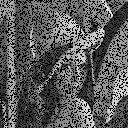
\includegraphics{Images/0.png}
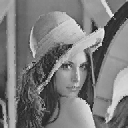
\includegraphics{Images/3.png}
\caption{Corrupted signal $\bs y$ (left) and reconstructed signal $\hat{\bs x}$ (right) using a cascade of 3 RVMs with Haar basis functions (see \cite{pilikos2014}).}
\label{fig:lennareconstruction}
\end{figure}

Apart from achieving sparse solutions, one further desirable feature of the RVM is that the model provides error bars for its predictions.
This is used in \cite{pilikos2014} to construct a multi-scale cascade of RVM estimations and achieve significant performance boosts.

An example of this can be seen in Figure \ref{fig:lennareconstruction}.

